\documentclass{beamer}
\beamertemplatenavigationsymbolsempty
\usecolortheme{beaver}
\setbeamertemplate{blocks}[rounded=true, shadow=true]
\setbeamertemplate{footline}[page number]
%
\usepackage[utf8]{inputenc}
\usepackage[english,russian]{babel}
\usepackage{amssymb,amsfonts,amsmath,mathtext}
\usepackage{subfig}
\usepackage[all]{xy} % xy package for diagrams
\usepackage{array}
\usepackage{multicol}% many columns in slide
\usepackage{hyperref}% urls
\usepackage{hhline}%tables
% Your figures are here:
\graphicspath{ {fig/} {../fig/} }

\begin{document}
\begin{frame}{Выбор интерпретируемых сверточных моделей глубокого обучения}

Рассматривается задача построения интерпретируемой сверточной нейронной сети. Под интерпретируемостью понимается выделение наиболее важных признаков и классификация схожих объектов одними и теми же классификаторами.

\begin{columns}[c]
\column{0.6\textwidth}
 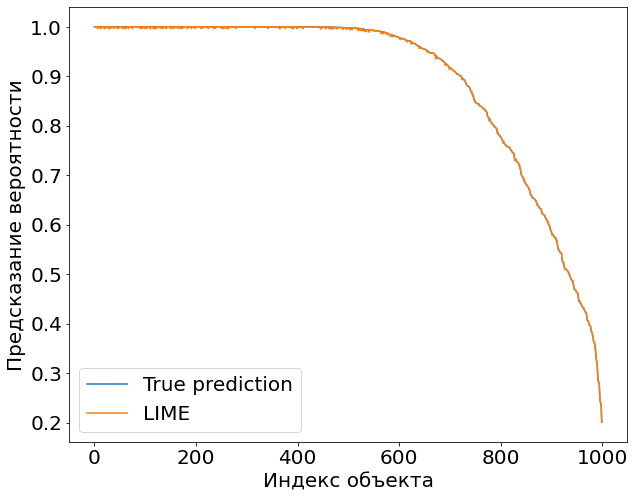
\includegraphics[width=0.75\textwidth]{../fig/lime_and_true.png}
\column{0.4\textwidth}
    Пакет LIME показывает хорошие результаты, попробуем их превзойти.
\end{columns}

\bigskip
К модели выдвигаются два требования: {\color{red}точность} и {\color{red}консистентность}.
\end{frame}

\end{document} 